% Author biographies. Photos live in figures/authors/.
% Five of the six photos are labelled placeholders; replace them with real
% portraits (1in wide, 1.25in tall) before submission.
%
% Facts for the two senior authors are taken from their institutional pages
% and the IEEE Fellow class lists. The Das entry draws on the Jadavpur
% University institutional repository, the author metadata of a 2026 npj
% Systems Biology paper, and WIPO. Note: a PhD and the job titles "Principal"
% or "Lead AI Scientist" appear on his own GitHub and LinkedIn profiles but on
% no independent source, so neither is stated here. The three remaining junior
% entries are deliberately thin: no degree year, title, or honour could be
% verified from a citable source, so those entries state only affiliation and
% research area and need each author to complete them.

\begin{IEEEbiography}[{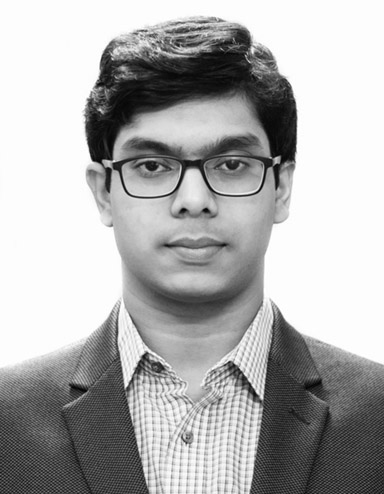
\includegraphics[width=1in,height=1.25in,clip,keepaspectratio]{figures/authors/rangan-das.jpg}}]{Rangan Das}
received the M.E. degree in computer science and engineering from Jadavpur University, Kolkata, India, in 2019, with a dissertation on fuzzy dilation and pooling in deep convolutional networks. He is currently with GeneSilico Inc., Austin, TX, USA, and the Department of Computer Science and Engineering, Jadavpur University. His research interests include deep learning, graph neural networks, biomedical image analysis, and agentic large language models for precision oncology. His work has appeared in ACM Computing Surveys, IEEE Transactions on Artificial Intelligence, Computers in Biology and Medicine, and npj Systems Biology and Applications, and he is a co-inventor on a pending patent application on computational modeling for personalized breast cancer treatment.
\end{IEEEbiography}

\begin{IEEEbiography}[{
\includegraphics[width=1in,height=1.25in,clip,keepaspectratio]{figures/authors/sounak-ghosh.jpg}}]{Sounak Ghosh}
received the B.E. degree in computer science and engineering from Jadavpur University, Kolkata, India, in 2025. His research interests include machine learning and knowledge-graph-based retrieval.
\end{IEEEbiography}

\begin{IEEEbiography}[{
\includegraphics[width=1in,height=1.25in,clip,keepaspectratio]{figures/authors/utsav-bandyopadhyay-maulik.jpg}}]{Utsav Bandyopadhyay Maulik}
is with the School of Computing, National University of Singapore, Singapore. His research interests include natural language processing, speech recognition, and machine learning for biomedical applications.
\end{IEEEbiography}

\begin{IEEEbiography}[{
\includegraphics[width=1in,height=1.25in,clip,keepaspectratio]{figures/authors/sushmit-dasgupta.jpg}}]{Sushmit Dasgupta}
received the B.E. degree in computer science and engineering from Jadavpur University, Kolkata, India. His research interests include machine learning and its application to biomedical data.
\end{IEEEbiography}

\begin{IEEEbiography}[{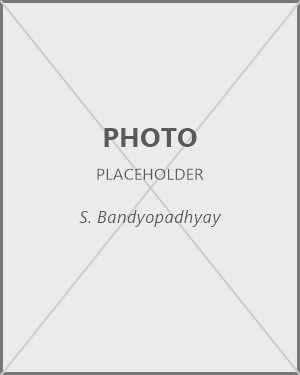
\includegraphics[width=1in,height=1.25in,clip,keepaspectratio]{figures/authors/sanghamitra-bandyopadhyay.jpg}}]{Sanghamitra Bandyopadhyay}
(Fellow, IEEE) received the Ph.D. degree from the Indian Statistical Institute, Kolkata, India, in 1998, where she is currently a Professor with the Machine Intelligence Unit and served as Director from 2015 to 2025. Her research interests include machine learning, evolutionary computation, pattern recognition, and computational biology, and her awards include the Shanti Swarup Bhatnagar Prize, the Infosys Prize, and the Padma Shri.
\end{IEEEbiography}

\begin{IEEEbiography}[{
\includegraphics[width=1in,height=1.25in,clip,keepaspectratio]{figures/authors/ujjwal-maulik.jpg}}]{Ujjwal Maulik}
(Fellow, IEEE) received the Ph.D. degree in engineering from Jadavpur University, Kolkata, India, in 1997, where he is currently a Professor with the Department of Computer Science and Engineering and a former Head of the same department. His research interests include machine learning, data science, computational biology and bioinformatics, and multi-objective optimization, and he is a Fellow of INAE, NASI, and the IAPR.
\end{IEEEbiography}
